% Aufbau
\subsection{Aufbau eines Radar}

Die folgende schematische Darstellung des Aufbaus eines Puls-Doppler-Radars (vgl. Abbildung \ref{fig:Aufbau}) ist stark vereinfacht und auf das Projekt angepasst. Eine ausführlichere Darstellung der Komponenten eines Radars ist beispielsweise in \cite[Abschnitt 1.4]{Ludloff} oder \cite[Abschnitt 1.3]{Richards} zu finden. 

\begin{figure}[h] 
  \centering
  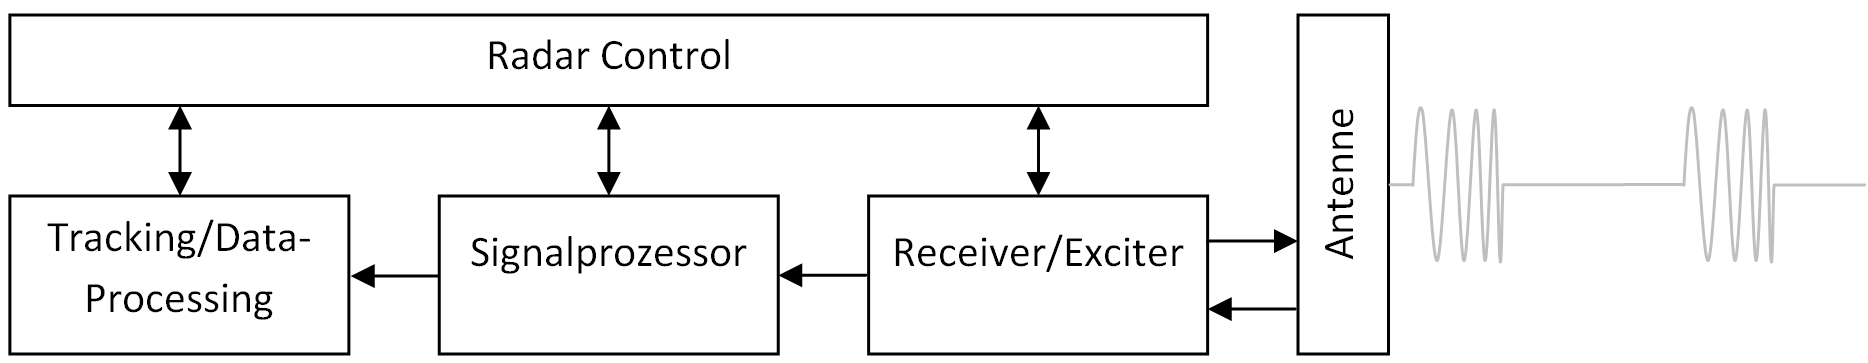
\includegraphics[scale=0.4]{images/Radar_Aufbau_Zoom240.PNG}
  \caption{Schematische Darstellung des Aufbaus eines Radars}
  \label{fig:Aufbau}
\end{figure}

Die Antenne sendet und empfängt elektromagnetische Signale. Diese beiden Phasen (Senden und Empfangen) laufen zyklisch, aber zeitlich getrennt voneinander ab, sodass beim Puls-Doppler-Radar eine Antenne ausreicht. Für das Aussenden der Signale wird der Exciter benötigt. Dieser erzeugt das Sendesignal, verstärkt es und mischt es vom sogenannten \glqq Basisband\grqq ~auf das \glqq Hochfrequenzband\grqq ~hoch (mehr dazu im folgenden Unterkapitel \ref{subsec:Signale}. Ist die Antenne auf Empfang geschaltet, so wird der Receiver aktiv. Dieser verstärkt und filtert  die empfangenen Signale und mischt sie auf das Basisband herunter (auch hierzu ist Genaueres in Kapitel \ref{subsec:Signale} zu finden. Der Receiver übernimmt des Weiteren die Aufgabe der Digitalisierung der bis dato analogen Daten. Die digitalisierten Daten werden im Signalprozessor weiterverarbeitet und analysiert. Ziel der Signalverarbeitung ist die Detektion von Zielen, sowie die Berechnung der Geschwindigkeiten, mit denen sich die Ziele fortbewegen. Beim Tracking/Data Processing werden die Detektionen weiterverarbeitet. Der gesamte Prozess wird durch die Radar Control gesteuert und koordiniert.